% Part: sets-functions-relations
% Chapter: arithmetization
% Section:reals

\documentclass[../../../include/open-logic-section]{subfiles}

\begin{document}

\olfileid{sfr}{arith}{real}
\olsection{वास्तव संख्या-रेषा}

पुढील पायरी म्हणजे परिमेय संख्यांपासून वास्तव संख्यांची रचना कशी करायची
हे दाखवणे. त्याआधी वास्तव संख्यांचे \emph{वैशिष्ट्य} नेमके काय आहे हे
समजून घ्यावे लागेल.

वास्तव संख्या परिमेय संख्यांसारख्याच बऱ्याच अंशी वागतात. (तांत्रिक
भाषेत, दोन्ही \emph{क्रमित क्षेत्रांची} उदाहरणे आहेत; त्याची व्याख्या
\olref[check]{orderedfield} मध्ये पाहा.) आता, तुम्ही \olref[sfr][siz][]{chap}
मधील सराव सोडवले असतील, तर वास्तव संख्या परिमेय संख्यांपेक्षा काटेकोरपणे
अधिक आहेत, म्हणजे $\cardless{\Rat}{\Real}$, हे तुम्हाला माहीत असेल.
हे कँटर यांनी प्रथम सिद्ध केले. परंतु अपरिमेय संख्या, म्हणजे परिमेय
नसलेल्या वास्तव संख्या, अस्तित्वात आहेत हे सुमारे अडीच सहस्रकांपासून
माहीत आहे. खरे तर:
%\footnote{टीप: पारंपरिक संकेतानुसार ``$\sqrt{2}$'' धन वर्गमूळ दर्शवते; पुढील काही पृष्ठांत आपण तेच मूळ विचारात घेऊ.}
%READERNOTE{MRARITH-002: गोठवलेल्या इंग्रजीतील निष्क्रिय केलेली तळटीप √2 हे धन आणि ऋण अशी दोन्ही मुळे दर्शवते असे म्हणते. पारंपरिक मूलचिन्ह मात्र मुख्य, ऋणेतर वर्गमूळ दर्शवते; म्हणून मराठीतील निष्क्रिय तळटीप दुरुस्त केली आहे. सक्रिय वाचनीय मजकुरावर याचा परिणाम नाही.}
\begin{thm}\ollabel{root2irrational}
$\sqrt{2}$ ही परिमेय संख्या नाही; म्हणजे $\sqrt{2} \notin \Rat$.
\end{thm}

\begin{proof}
व्याघातासाठी $\sqrt{2}$ ही परिमेय संख्या आहे असे समजा. मग काही नैसर्गिक
संख्या $m$ आणि $n$ यांसाठी $\sqrt{2} = \nicefrac{m}{n}$. हा अपूर्णांक
यापुढे संक्षिप्त करता येणार नाही अशा रीतीने आपण $m$ आणि $n$ निवडू शकतो.
पुनर्मांडणी केल्यास $m^{2} = 2n^{2}$. येथून सिद्धता दोन प्रकारे पूर्ण
करता येते:

\emph{प्रथम, भूमितीय रीतीने} (टेनेनबाउम यांच्या पद्धतीने).\footnote{ही
सिद्धता \cite{Conway2006} यांनी नोंदवली आहे.} पुढील चौरस पाहा:
\begin{center}
	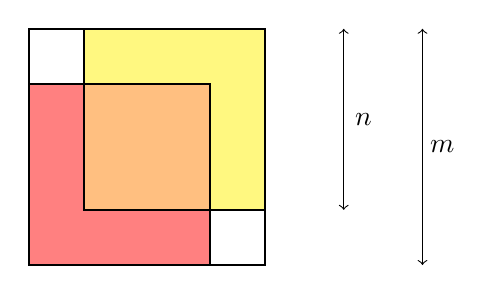
\begin{tikzpicture}
		\draw[thick] (0,0) rectangle (3,3);
		\draw[thick, fill=red!50] (0,0) rectangle (2.3,2.3);
		\draw[thick, fill=yellow!50] (0.7,0.7) rectangle (3, 3);
		\draw[thick, fill=orange!50] (0.7,0.7) rectangle (2.3, 2.3);
		\draw[<->] (4, 0.7)--(4, 3);
		\node at (4.25, 1.85) (n) {$n$};
		\draw[<->] (5, 0)--(5, 3);
		\node at (5.25, 1.5) (m) {$m$};
	\end{tikzpicture}
\end{center}
$m^2 = 2n^2$ असल्यामुळे $n$ बाजू असलेले दोन चौरस ज्या प्रदेशात
एकमेकांवर येतात त्याचे क्षेत्रफळ, या दोन्ही चौरसांपैकी एकानेही न झाकलेल्या
प्रदेशाच्या क्षेत्रफळाइतके आहे; म्हणजे नारिंगी चौरसाचे क्षेत्रफळ हे दोन
न रंगवलेल्या चौरसांच्या क्षेत्रफळांच्या बेरजेइतके आहे. नारिंगी चौरसाची
बाजू $p$ आणि प्रत्येक न रंगवलेल्या चौरसाची बाजू $q$ असेल, तर $p^2 =
2q^2$. पण आता $p < m$, $q < n$ आणि $p, q \in \Nat$ असून
$\sqrt{2} = \nicefrac{p}{q}$. हे $m$ आणि $n$ शक्य तितके लहान निवडले
होते या तथ्याशी विसंगत आहे.

\emph{दुसरी, आकारिक रीतीने.} $m^{2} = 2n^{2}$ असल्यामुळे $m$ सम आहे.
($x$ विषम असेल, तर $x^2$ विषम असतो हे सहज दाखवता येते.) म्हणून काही
$r \in \Nat$ साठी $m = 2r$. पुनर्मांडणी केल्यास $2r^2 = n^2$,
		% 			\begin{align*}
		% 				(2q)^{2} &= 2n^{2}\\
		% 				4q^{2} &= 2n^{2}\\
		% 				2q^{2} &= n^{2}
		% 			\end{align*}
त्यामुळे $n$ देखील सम आहे. म्हणून $m$ आणि $n$ दोन्ही सम आहेत, आणि
त्यामुळे $\nicefrac{m}{n}$ हा अपूर्णांक पुढे \emph{संक्षिप्त करता येतो}.
व्याघात!
\end{proof}

जाताजाता, या आकृतीवरील सिद्धतेमुळे \olref[his][set][mythology]{sec}
मधील सामग्रीचा पुन्हा विचार करता येतो. टेनेनबाउम (1927--2005) हे पूर्णपणे
आधुनिक गणितज्ञ होते; तरी ही सिद्धता निर्विवादपणे सुंदर, पूर्णतः तर्कशुद्ध
आहे आणि भूमितीय अंतःप्रज्ञेला आवाहन करते!
%READERNOTE{MRARITH-003: गोठवलेल्या इंग्रजी मजकुरात निधनवर्ष 2006 दिले आहे. टेनेनबाउम यांच्या स्मृतिस्थळावरील चरित्र नोंद निधनाची तारीख 4 मे 2005 देते; मराठी मजकुरात 1927--2005 वापरले आहे.}

कसेही असो, वास्तव संख्या परिमेय संख्यांपेक्षा ``अधिक विस्तृत'' आहेत.
एका अर्थाने परिमेय संख्यांमध्ये ``पोकळ्या'' आहेत आणि वास्तव संख्या त्या
भरून काढतात. वायश्ट्रास यांच्या लक्षात आले की या वर्णनातून वास्तव
संख्यांचा एकच गुणधर्म व्यक्त होतो, जो त्यांना परिमेय संख्यांपासून वेगळे
करतो; तो म्हणजे संपूर्णता गुणधर्म: \emph{ऊर्ध्वबंध असलेल्या वास्तव
संख्यांच्या प्रत्येक अरिक्त संचाला लघुतम ऊर्ध्वबंध असतो.}

परिमेय संख्यांना संपूर्णता गुणधर्म नाही हे सहज दिसते. उदाहरणार्थ,
$\sqrt{2}$ पेक्षा लहान परिमेय संख्यांचा पुढील संच पाहा:
\[
	\Setabs{p \in \Rat}{p^2 < 2 \text{ किंवा }p < 0}
\]
या संचाला परिमेय संख्यांमध्ये ऊर्ध्वबंध आहे; उदाहरणार्थ, त्याचे सर्व
!!{element}s< $3$ पेक्षा लहान आहेत. पण त्याचा लघुतम ऊर्ध्वबंध कोणता?
आपल्याला ` $\sqrt{2}$ ' असे म्हणायचे आहे; पण $\sqrt{2}$ ही \emph{परिमेय
संख्या नाही} हे आपण नुकतेच पाहिले. आणि $\sqrt{2}$ पेक्षा मोठी अशी कोणतीही
\emph{लघुतम} परिमेय संख्या नाही. म्हणून या संचाला ऊर्ध्वबंध आहे, पण लघुतम
ऊर्ध्वबंध नाही. त्यामुळे परिमेय संख्यांमध्ये संपूर्णता गुणधर्माचा अभाव आहे.

याउलट, सांतत्याला संपूर्णता गुणधर्म स्वभावतः असायला हवा. $\sqrt{2}$ ही
केवळ वास्तव संख्या असावी एवढेच आपल्याला नको; परिमेय संख्या-रेषेतील सर्व
``पोकळ्या'' भरायच्या आहेत. खरे तर सांतत्यात स्वतःमध्येच कोणतीही ``पोकळी''
नसावी असे आपल्याला हवे आहे. संपूर्णतेद्वारे नेमके हेच मिळेल.

\end{document}
